\section{Key-Value Cache (KV Cache)}

The Primary Goal of a Transformer during inference is to generate One Token at a time. This Process is Known as autoregressive Generation, Meaning that each newly generated Token depends on all Previously generated tokens.

Unlike training, where the entire target Sequence is available simultaneously, inference has access only to The Tokens that have already been Generated, Therefore, The model must repeatedly execute the decoder every new token until the Sequence is complete.

Suppose we want The model to Generate the Sentence: \\


\textit{The cat is sleeping on the sofa.}

\begin{center}
\begin{tabular}{l l}
$\langle \text{BOS} \rangle$
& $\rightarrow$ Predict ``The'' \\[4pt]

$\langle \text{BOS} \rangle$ The
& $\rightarrow$ Predict ``cat'' \\[4pt]

$\langle \text{BOS} \rangle$ The cat
& $\rightarrow$ Predict ``is'' \\[4pt]

$\langle \text{BOS} \rangle$ The cat is
& $\rightarrow$ Predict ``sleeping'' \\[4pt]

$\langle \text{BOS} \rangle$ The cat is sleeping
& $\rightarrow$ Predict ``on'' \\[4pt]

$\langle \text{BOS} \rangle$ The cat is sleeping on
& $\rightarrow$ Predict ``the'' \\[4pt]

$\langle \text{BOS} \rangle$ The cat is sleeping on the
& $\rightarrow$ Predict ``sofa'' \\[4pt]

$\langle \text{BOS} \rangle$ The cat is sleeping on the sofa
& $\rightarrow$ $\langle \text{EOS} \rangle$
\end{tabular}
\end{center}

Notice that The input sequence grows after every generation step, At step $t$, The decoder receives all Tokens Generated up to step $t-1$.

\subsection{The Central Idea behind KV Cache}

The Central Idea behind KV cache is simple but Powerful: Previous token never change after They are generated, Consequently, their Key and Value vectors remain Constant and do not need to be recomputed.

By storing these vectors in memory and reusing them at every generation step, the decoder avoids redundant computation and computes the query, key, and value only for the newest token. This optimization dramatically accelerates inference while producing exactly the same output as the original Transformer without caching.

Understanding the KV cache begins with recognizing the fundamental difference between training and inference.

\paragraph{During Training}
The model already knows the complete target sentence because it is provided by the training dataset. Using teacher forcing, the entire shifted target sequence is fed into the decoder simultaneously. For example, if the target sentence is ``The cat is sleeping,'' the decoder receives $\langle \text{BOS} \rangle$ ``the cat is sleeping'' in a single forward pass. Because all tokens are processed in parallel, the Transformer computes attention for every position at once.

\paragraph{During Inference}
The future words are unknown. The decoder initially receives only $\langle \text{BOS} \rangle$ and predicts the first token. It runs again for each generated token, performing $n$ separate forward passes. The computational cost therefore increases with sequence length, and this repeated computation becomes the primary bottleneck during inference.

\subsection{The Motivation for KV Cache}

The key observation behind the KV cache is that previously generated tokens do not change during autoregressive generation. Once a token has been processed, its key and value vectors remain constant and are identical in all subsequent decoding steps.

\paragraph{Example (Without KV Cache)}
\begin{itemize}
    \item Step 1: Compute $Q, K, V$ for token 1
    \item Step 2: Compute $Q, K, V$ for token 1 and 2
    \item Step 3: Compute $Q, K, V$ for tokens 1 and 2 and 3
\end{itemize}

The KV cache eliminates this inefficiency by storing the computed key and value vectors in memory. During subsequent decoding steps, the model reuses the cached keys and values and computes new projections only for the most recently generated token. The query vector is not cached because it is always computed from the current token being processed.

\paragraph{After Using the KV Cache}
\begin{itemize}
    \item Step 1: Compute $Q$, $K$, and $V$ for token 1; store $K$ and $V$.
    \item Step 2: Compute $Q$, $K$, and $V$ for token 2; reuse the $K$ and $V$ of token 1, then store those of token 2.
    \item Step 3: Compute $Q$, $K$, and $V$ for token 3; reuse the $K$ and $V$ of tokens 1 and 2, then store those of token 3.
\end{itemize}

The decoder no longer recomputes Keys and Values for Previous tokens.

This optimization Produces exactly The Same model Output as the Original Transformer while Significantly reducing The Computational Cost of autoregressive inference, making real-time text Generation Practical for modern Large language models.

\subsection{Equation \& Complexity}

The new Equation becomes:
\begin{equation}
\text{Attention} = \text{Softmax}\left(\frac{Q_t K_{\text{cache}}^T}{\sqrt{d_k}}\right) \cdot V_{\text{cache}}
\end{equation}

\begin{align*}
K_{\text{cache}} &\in \mathbb{R}^{B \times h \times L \times d_k} \\
V_{\text{cache}} &\in \mathbb{R}^{B \times h \times L \times d_k}
\end{align*}
$B$: Batch size, $h$: N. of heads, $L$: Sequence length, $d_k$: Head dimention.

\paragraph{Complexity}
\begin{itemize}
    \item Without KV cache: $\mathcal{O}(n^2)$
    \item With KV cache: $\mathcal{O}(n)$
\end{itemize}

KV cache exchange Computation for memory, The memory needs to grows linearly with the Context length:
\begin{equation}
\text{Memory} = 2 B h L d_k
\end{equation}
(Key, Value)

As the context length increase, The cache Consumes more Gpu memory (VRAM) which becomes one of The Primary limitations of long-context language Models.

\paragraph{Advantages}
\begin{itemize}
    \item Eliminates redundant computation of Previously generated Keys and Values
    \item Significantly accelerates autoregressive (generate one token at time) inference
    \item Reduces Computational Complexity and Key, value Projection from $\mathcal{O}(n^2)$ to $\mathcal{O}(n)$
    \item Produces exactly The Same outputs as the Original Transformer without caching
    \item Used by virtually all modern decoder-only Large language models
\end{itemize}

\paragraph{Limitation}
\begin{itemize}
    \item Requires additional Gpu memory (vRAM) to Store The cache
    \item The Memory consumption increase linearly with the context length
    \item Does not improve training Speed because memory-bound due to the large cache size
\end{itemize}

\section{Modern Variants of KV Cache}

\subsection{I) Multi-Query Attention (MQA)}

\paragraph{Motivation} In standard multi-head attention, every attention head has its own query, key, and value projections. Consequently, each head requires its own key and value cache, leading to high memory consumption during inference.

MQA reduces memory overhead by allowing all attention heads to share a single key projection and a single value projection, while each head retains its own query projection.

\paragraph{Instead of}
\begin{align*}
\text{Head 1} &\longrightarrow Q_1, K_1, V_1 \\
\text{Head 2} &\longrightarrow Q_2, K_2, V_2 \\
&\;\;\dots \\
\text{Head } h &\longrightarrow Q_h, K_h, V_h
\end{align*}

\paragraph{MQA becomes}
\begin{align*}
\text{Head 1} &\longrightarrow Q_1 \\
\text{Head 2} &\longrightarrow Q_2 \\
&\;\;\dots \\
\text{Head } h &\longrightarrow Q_h \\
&\quad (\text{Shared } K \text{ and } V)
\end{align*}

\begin{figure}[H]
    \centering
    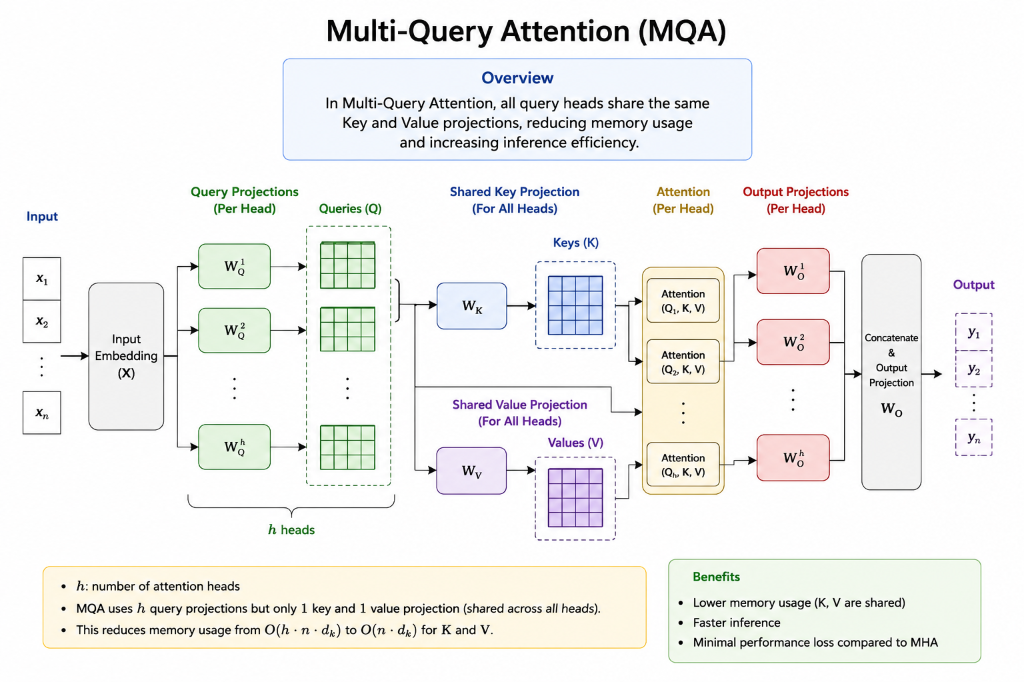
\includegraphics[width=0.95\textwidth]{figures/fig_5_1_gqa.png}
    \caption{Multi-Query Attention (MQA)}
    \label{fig:5_7_mqa}
\end{figure}

\paragraph{Advantages}
\begin{itemize}
    \item Much smaller KV cache
    \item Lower Gpu memory usage
    \item Faster inference
    \item Particularly effective for very LLMs
\end{itemize}

\paragraph{Limitation} Sharing a Single Key and Value across all heads slightly reduces The representational Capacity of The Attention mechanism.

\subsection{II) Grouped-Query Attention (GQA)}

\paragraph{Motivation} MQA greatly reduces memory usage but may sacrifice some modeling capacity because all heads share the same key and value.

GQA provides a compromise between standard multi-head attention and MQA.

\paragraph{Architecture} Instead of one key and value per head or one shared key and value for all heads, attention heads are divided into groups.

Each group shares a key and value projection.

\paragraph{For example} Eight query heads and two KV groups:
\begin{itemize}
    \item Heads 1 to 4: shared $K_1$ and shared $V_1$
    \item Heads 5 to 8: shared $K_2$ and shared $V_2$
\end{itemize}

\begin{figure}[H]
    \centering
    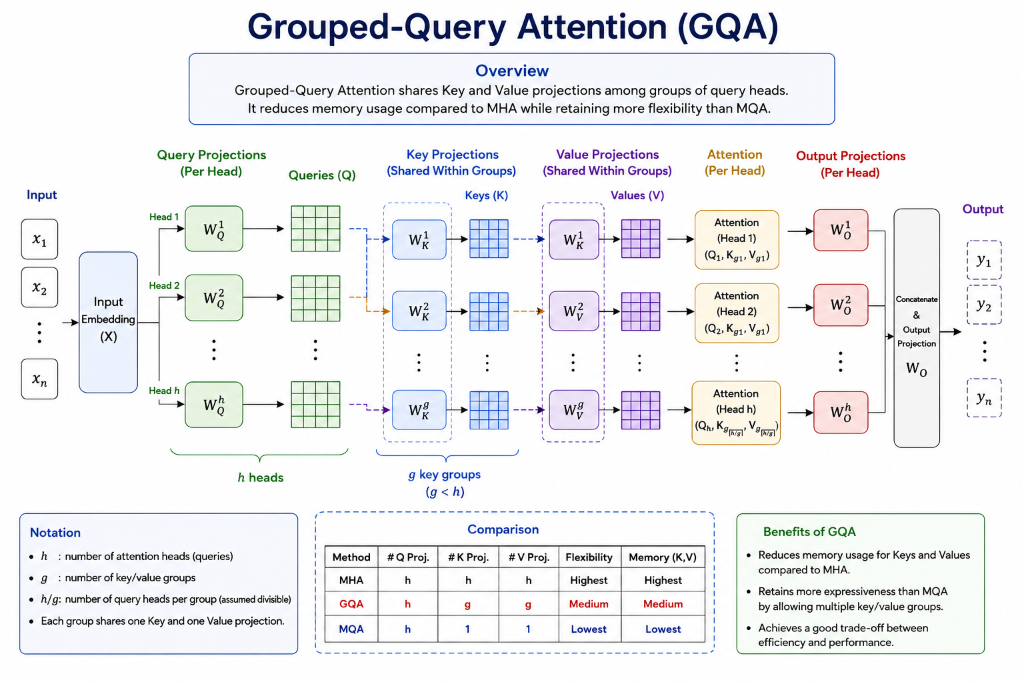
\includegraphics[width=0.95\textwidth]{figures/fig_5_1_mla.png}
    \caption{Grouped-Query Attention (GQA)}
    \label{fig:5_8_gqa}
\end{figure}

\paragraph{Advantages}
\begin{itemize}
    \item Smaller KV cache than Standard Multi-Head Attention
    \item Better modeling capacity than MQA
    \item Excellent balance between memory efficiency and model quality
    \item Widely adopted in modern LLMs
\end{itemize}

\paragraph{Limitation} Although much smaller than standard Multi-Head Attention, The cache remains larger than in MQA.

\subsection{III) Multi-Head Latent Attention (MLA) DeepSeek}

This is currently one of the biggest innovation.

Instead of Storing Keys and Values directly, DeepSeek stores a Compressed latent representation.

\begin{center}
Token $\longrightarrow$ Latent Compression $\longrightarrow$ Small Latent Vector $\longrightarrow$ Cache Latent $\longrightarrow$ when needed Reconstruct $K, V$
\end{center}

So instead of Store $K$ and $V$, DeepSeek stores $z$ (latent vector).

\begin{itemize}
    \item $K$: 512 number, $V$: 512 number, store: 1024 numbers
    \item Latent $\longrightarrow$ 128 numbers
\end{itemize}

Memory is dramatically reduced.

\begin{figure}[H]
    \centering
    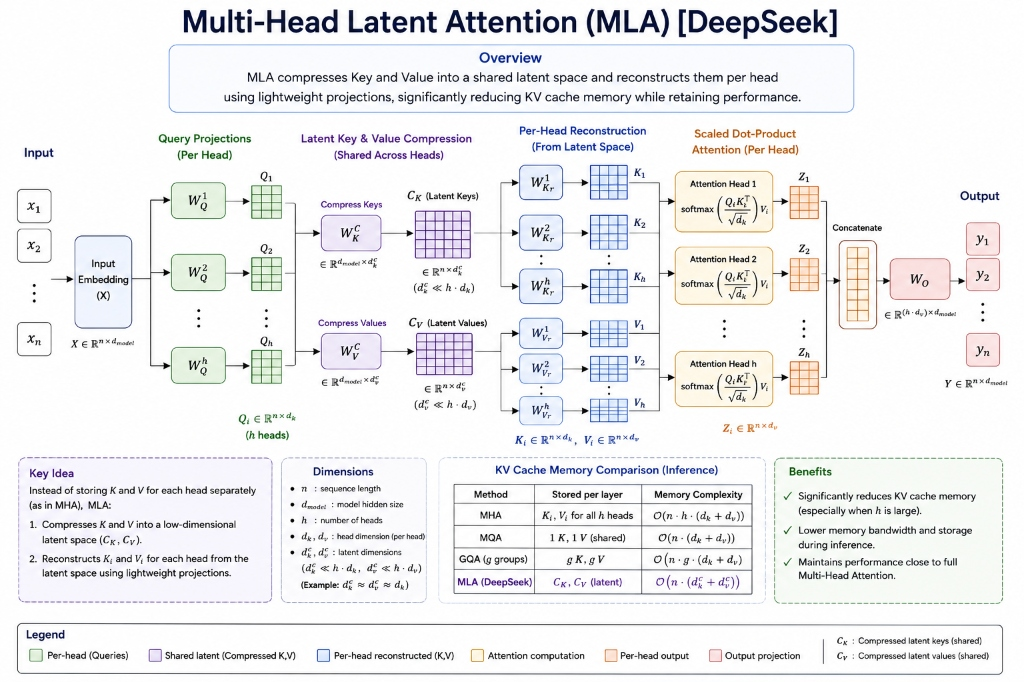
\includegraphics[width=0.98\textwidth]{figures/fig_5_1_comparison.jpg}
    \caption{Multi-Head Latent Attention (MLA) [DeepSeek]}
    \label{fig:5_9_mla}
\end{figure}

\paragraph{Advantages}
\begin{itemize}
    \item Much smaller Kv cache
    \item Longer Context
    \item Better Than GQA for memory
    \item Lower VRAM
    \item Faster inference
\end{itemize}

\begin{figure}[H]
    \centering
    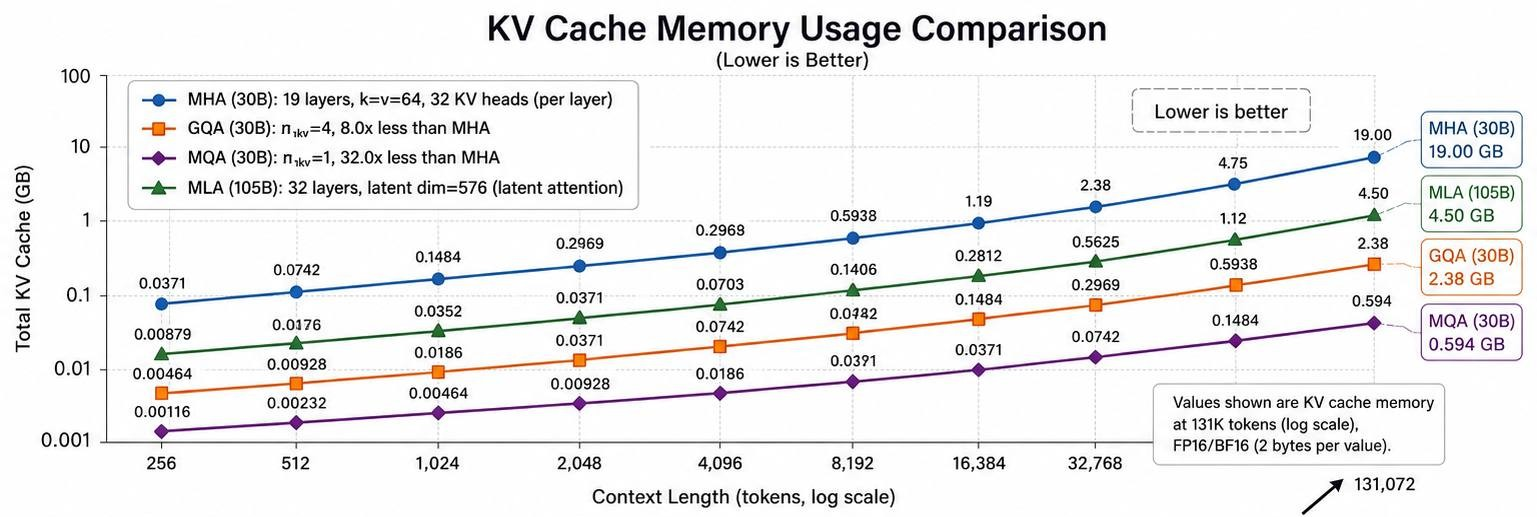
\includegraphics[width=0.95\textwidth]{figures/kv1.jpg}
    \caption{KV Cache Memory Usage Comparison}
    \label{fig:5_6_comparison}
\end{figure}

\begin{figure}[H]
    \centering
    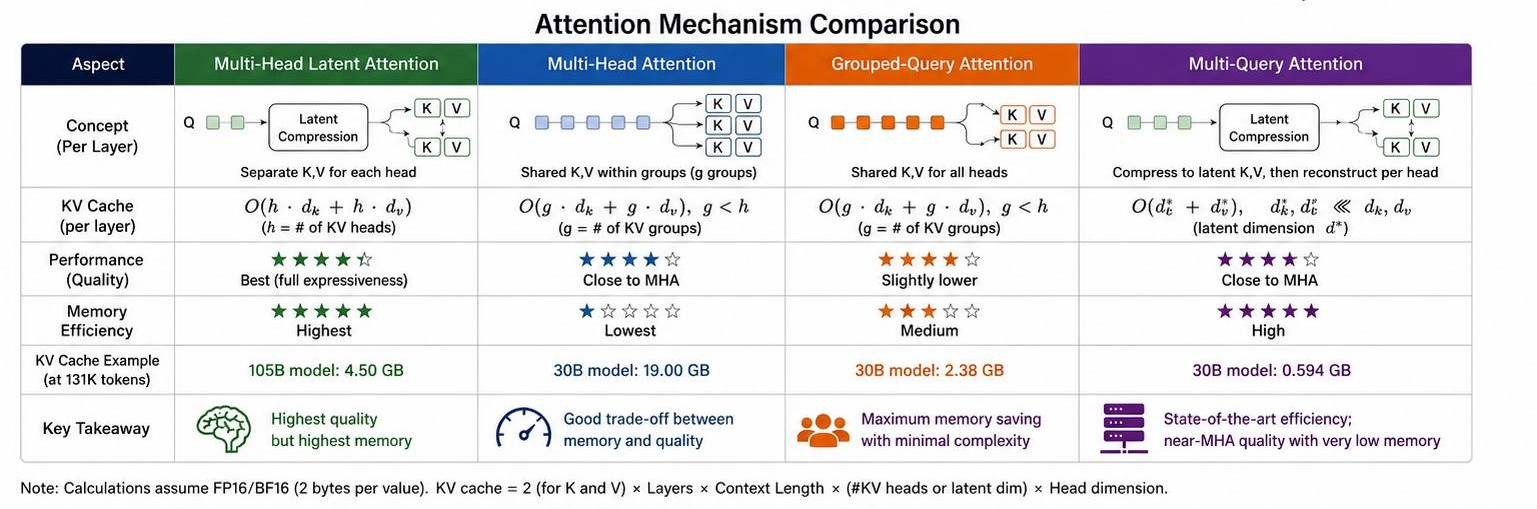
\includegraphics[width=0.95\textwidth]{figures/kv2.jpg}
\end{figure}
\section{Encoder-Only Transformers (BERT Family)}

The Original Transformer was designed for Seq2Seq tasks, where both an encoder and a decoder are required. However, many NLP applications require only language understanding and Never generate new Text as:
\begin{itemize}
    \item Text Classification
    \item Sentiment Analysis
    \item Named Entity Recognition (NER)
    \item Spam detection
    \item Semantic Similarity
    \item Document Classification
\end{itemize}

The Original Transformer (Encoder-Decoder) was Specifically designed for Seq2Seq tasks as machine translation. The researchers recognized That The encoder alone already Produces rich Contextual representations of the input Sequence. Every Encoder layer allows each token to Attend to every other token through bidirectional Self Attention, Producing Contextual embeddings that Capture both local and Global Semantic relationships.

Therefore, if The Goal is to understand text rather Than generate it, The encoder already Provides everything that is needed. This Observation led to a fundamental architecture simplification: Remove the decoder entirely and Retain only the encoder stack.

\subsection{BERT (Bidirectional Encoder Representation from Transformer)}

Based on This idea, Google introduced BERT in 2018 the first Large-scale Pretrained encoder-only Transformer.

BERT consists only of Input $\longrightarrow$ Encoder $\longrightarrow$ Task-specific Output Layer.

The decoder is Completely removed because BERT is designed for understanding rather than generation.

After Several encoder layer, every token contains information from The entire input Sequence. These Contextual embeddings Capture lexical meaning, syntax, semantics and long-range dependencies making them suitable for a wide variety of downstream NLP tasks.

Instead of Generating Text, BERT directly uses these Contextual Representations to make Predictions through a lightweight task-specific output layer.

\paragraph{BERT Architecture}
Unlike the Original Transformer encoder architecture, BERT introduces several modifications to The input representation and training procedure that enable it to learn deep bidirectional contextual representation from Large-scale unlabeled text.

The architecture primarily consists of stacked encoder blocks:
\begin{itemize}
    \item BERT-Base: 12 stacked encoder layers, 12 attention heads and 110 million parameters.
    \item BERT-Large: 24 stacked encoder layers, 16 attention heads and 340 million parameters.
\end{itemize}

BERT introduces a richer input representation by combining token, position, segment embedding:
\begin{equation}
E = E_{\text{token}} + E_{\text{pos}} + E_{\text{segment}}
\end{equation}

BERT Learns Positional Embeddings during Training and produces Contextual representations for every input token which are later used for various downstream NLP tasks.

\subsection{WordPiece Tokenization}

WordPiece Tokenization is a sub-word-based algorithm that enables BERT to efficiently represent text using a fixed-size Vocabulary. By decomposing words into smaller subword units, it Greatly reduces the out-of-vocabulary problem.

Suppose the Vocabulary contains: Play, Playing, Played, Player. Now consider the word playfulness if it not exist in the vocabulary, a word-level Tokenizer cannot represent it and replaces it with \texttt{[unk]}. As a result, all information contained in the word is lost, This Problem is Known as the Out-of-Vocabulary (OOV) problem.

Instead of treating every word as a unique token WordPiece decomposes words into smaller units:
\begin{align*}
\text{Playing} &\longrightarrow \text{Play}, \;\; \text{\#\#ing} \\
\text{Unbelievable} &\longrightarrow \text{un}, \;\; \text{\#\#believ}, \;\; \text{\#\#able}
\end{align*}

The Prefix ""\#\#"" indicates that the Subword Continues the Previous token rather than beginning a new word.

By combining a relatively small set of subwords, WordPiece can represent an enormous number of words, including many that were never seen during training.

Rather than Storing complete words, The Vocabulary contains frequent subwords learned from a large text Corpus. Typical entries include: Play, \texttt{\#\#er}, \texttt{\#\#ing}, \texttt{\#\#ed}, \texttt{\#\#able}, \texttt{\#\#tion}.

For English BERT, the vocabulary contains approximately 30,000 subword tokens. This vocabulary size provides a good balance between representation power and computational efficiency.

\paragraph{Tokenization Process}
The Player is unbelievable. $\longrightarrow$ The, Play, \texttt{\#\#er}, is, un, \texttt{\#\#believ}, \texttt{\#\#able}

Each subword is then mapped to an integer index, which is later converted into a dense embedding vector before entering The Transformer encoder.

If a word cannot be decomposed into Known subwords, it is replaced with The Special token \texttt{[unk]}. However, Because wordPiece can Construct most words from existing subwords, the occurence of \texttt{[unk]} is much lower than in word-level tokenization.

\subsection{Special Tokens and Input Representation}

BERT introduces several Special tokens that Provide structural information and Support different Pretraining and downstream tasks:

\begin{itemize}
    \item \texttt{[cls]}: The beginning of every input sequence, After passing through The encoder, the contextual representation of \texttt{[cls]} is considered a Summary of The entire input Sequence. Instead of Using all token embeddings, many downstream tasks use only The final hidden state of \texttt{[cls]}: $h_{\text{cls}} \in \mathbb{R}^{d_{\text{model}}}$. This vector is passed to a classifier for tasks such as:
    \begin{itemize}
        \item Sentiment Analysis
        \item Spam detection
        \item Topic classification
        \item Next Sentence Prediction
    \end{itemize}
    
    \item \texttt{[SEP]} token (Separator): Marks The end of a sentence or Separate two input sentences: \texttt{[cls]} Question? \texttt{[sep]} Answer \texttt{[sep]}
    
    \item \texttt{[Mask]} token: Is used only during Pretraining. A percentage of input tokens are replaced by \texttt{[mask]}, and The model learns to predict The original words using their surrounding context. \\
    ex: The cat is \texttt{[MASK]} target: Sleeping. \\
    This forms the basis of Masked Language Modeling (MLM) which allows BERT to learn bidirectional Contextual representations. During fine-tuning and inference, The \texttt{[MASK]} token is generally not present, except when performing masked-word prediction tasks.
    
    \item \texttt{[PAD]} token: When Sequences have different lengths, shorter sequences are padded using the \texttt{[PAD]} token.
    \begin{align*}
    \text{Sentence 1}: &\quad \texttt{[cls] I Love AI [SEP]} \\
    \text{Sentence 2}: &\quad \texttt{[cls] Hello . [SEP] [PAD] [PAD]}
    \end{align*}
    Padding ensures that all Sequences in the batch have identical dimension. During Attention computation, Padding tokens are ignored Through an attention mask, Preventing them from influencing the model's Predictions.
\end{itemize}

\subsection{Complete Input Pipeline}

The complete flow of text processing in BERT from raw string to encoder input is presented below:

\begin{figure}[H]
    \centering
    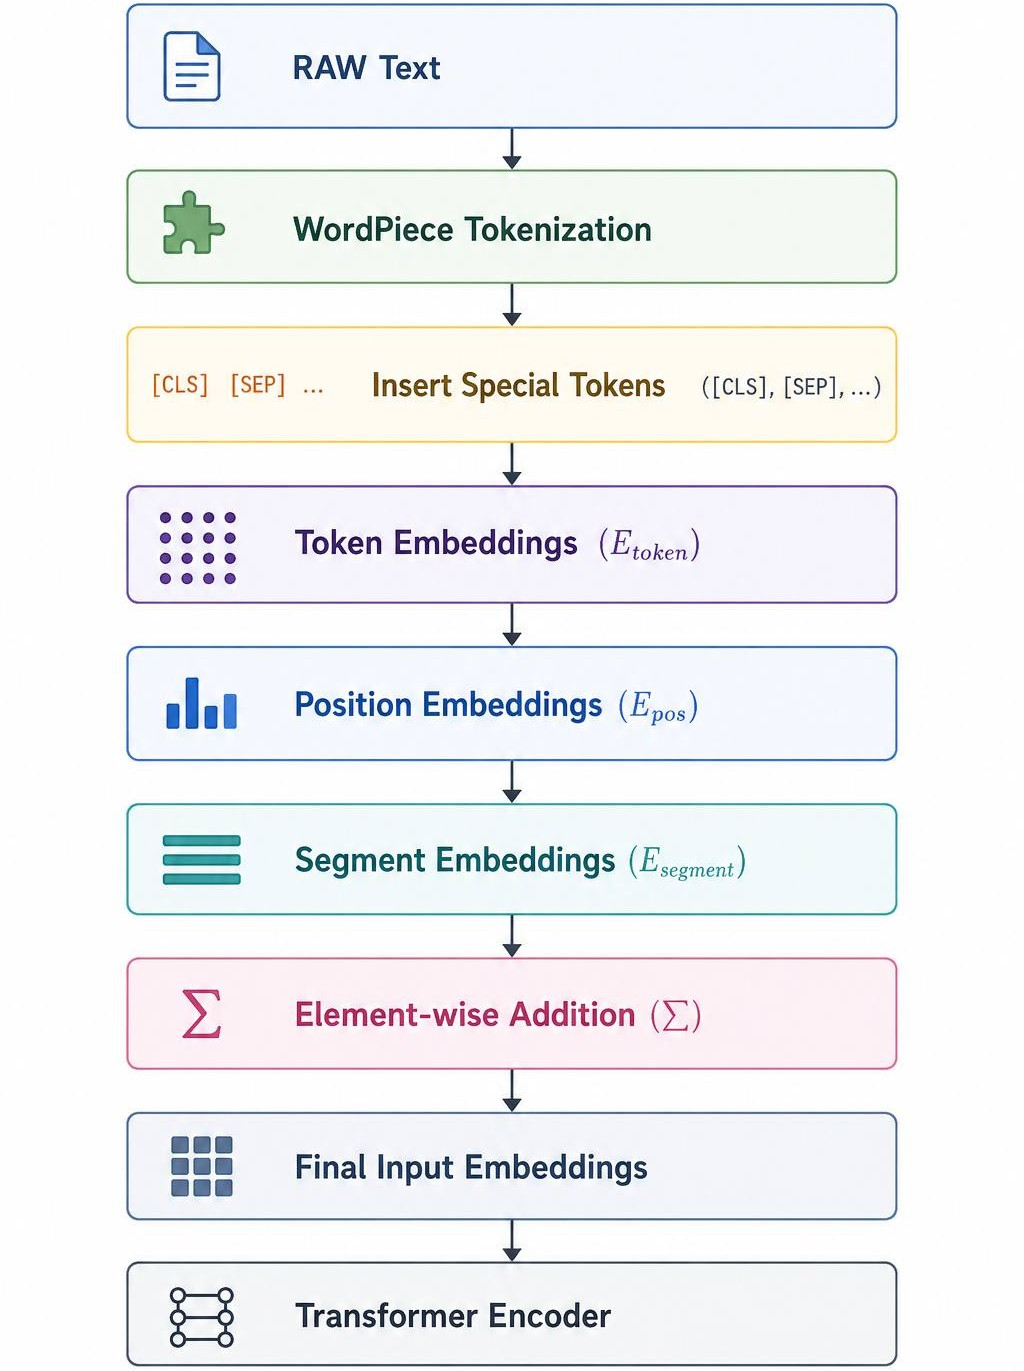
\includegraphics[width=0.95\textwidth]{figures/rnn1.jpg}
\end{figure}

\clearpage
\subsection{Bidirectional Learning}

The defining characteristic of BERT is its ability to learn bidirectional contextual representations. Unlike autoregressive language models, which process text from left to right, BERT simultaneously attends to both the left and right context of every token. This enables the model to construct richer semantic representations and achieve strong performance on language-understanding tasks.

Traditional autoregressive models predict the next token by Considering only the Previous tokens. In Contrast, BERT Processes the entire Sequence simultaneously. Every token can attend to every other token in The Sentence.

\subsection{Next Sentence Prediction (NSP)}

\paragraph{Motivation} Many NLP tasks require understanding the relationship between two sentences rather than a single sentence. Examples include question answering, natural language inference, and semantic similarity.

To Capture These inter-Sentence relationships, BERT introduces Next Sentence Prediction (NSP) as a Second Pretraining Objective.

\paragraph{Training Data Construction}
During Pretraining, The model receives pairs of Sentences.
\begin{itemize}
    \item $50\%$ of The pairs Contain two consecutive sentences from The Original Corpus ($\text{IsNext}$)
    \item $50\%$ Contain two randomly selected, unrelated sentences ($\text{NotNext}$). This creates a balanced binary classification problem.
\end{itemize}

This Creates a balanced binary Classification Problem.

\paragraph{Classification}
After passing through the encoder, the contextual representation of the \texttt{[CLS]} token, $h_{\text{cls}}$, is used as a representation of the entire sentence pair. A linear classifier predicts whether sentence B follows sentence A:
\begin{equation}
P(y) = \text{Softmax}(h_{\text{cls}} W + b)
\end{equation}

\paragraph{Loss function}
NSP is optimized using binary cross-entropy loss:
\begin{equation}
\mathcal{L}_{\text{NSP}} = -y \log(p) - (1-y) \log(1-p)
\end{equation}
\begin{itemize}
    \item $y=1$: for $\text{IsNext}$
    \item $y=0$: for $\text{NotNext}$
\end{itemize}

BERT is trained by optimizing both objectives simultaneously:
\begin{equation}
\mathcal{L} = \mathcal{L}_{\text{MLM}} + \mathcal{L}_{\text{NSP}}
\end{equation}
The encoder parameters are updated jointly using the combined loss.

\subsection{Limitations of NSP}

Subsequent research found that NSP contributed less than initially expected.

The RoBERTa model removed NSP entirely and achieved better performance by training longer on larger datasets.

Although NSP is no longer widely used in modern encoder models, it remains an important component of the original BERT architecture.

Thus, BERT learns both contextual word representations and sentence-level semantics. Although later models demonstrated that NSP is not essential, it played a significant role in the original BERT training procedure.

\subsection{Pretraining Summary}

Before BERT can be applied to downstream tasks such as sentiment analysis and question answering, it undergoes a large-scale pretraining phase. During this stage, the model learns general linguistic knowledge from massive collections of unlabeled text using the self-supervised objectives introduced in MLM (masked language modeling) and NSP (next-sentence prediction).

The result of pretraining is a model that captures grammar, semantics, contextual relationships, and sentence-level information, making it an effective starting point for many NLP applications.

\subsection{Fine-Tuning BERT}

Because BERT has already learned general language representations during pretraining, only a small amount of additional training is needed to specialize these representations for a specific task.

Rather than learning language from scratch, the model learns how to map its existing knowledge to the desired outputs.

Fine-tuning adapts a pretrained BERT model to a specific downstream task using labeled data. During training, both the encoder and the prediction head are optimized jointly, allowing the model to specialize its contextual representations while retaining the linguistic knowledge acquired during pretraining. This transfer-learning approach is one of the main reasons for BERT's effectiveness across a wide range of NLP tasks.

\paragraph{Fine-Tuning Pipeline}
The standard procedure for fine-tuning BERT on downstream tasks is illustrated below:
\begin{figure}[H]
    \centering
    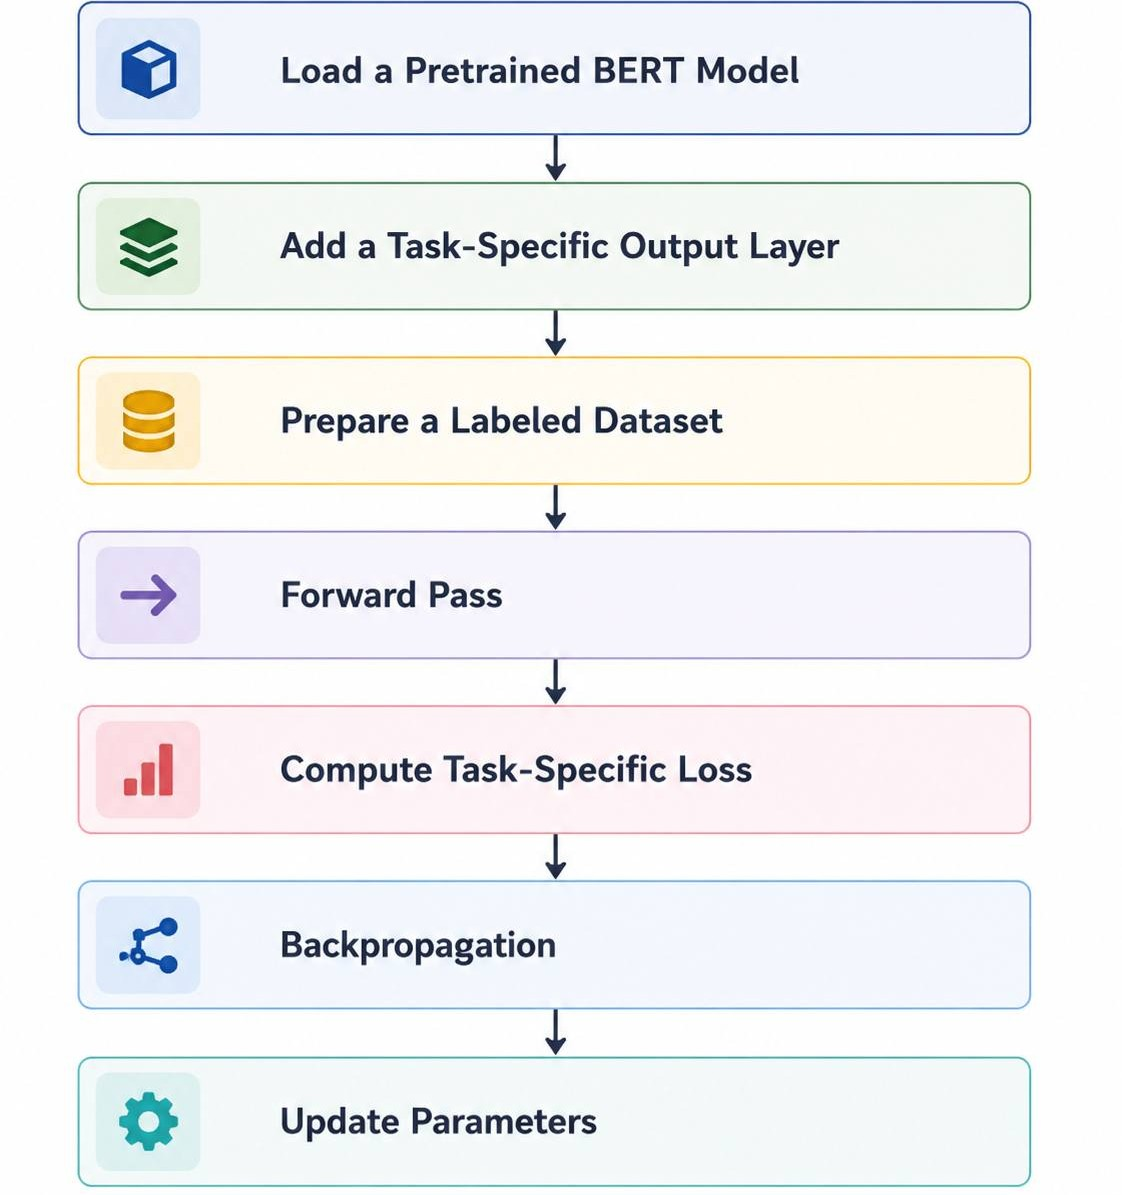
\includegraphics[width=0.95\textwidth]{figures/rnn2.jpg}
\end{figure}
\section{Decoder-Only Transformers (GPT Family)}

The decoder-only architecture emerged from the observation that many applications require only text generation or next-token prediction. The encoder becomes unnecessary, allowing the model to rely solely on the Transformer decoder. This simplification led to the GPT family of models, which has become the dominant architecture for modern large language models because of its scalability, simplicity, and effectiveness in autoregressive text generation.

\subsection{The Limitations of the Original Transformer}

Consider the task of machine Translation:
\begin{equation*}
\text{English} \longrightarrow \text{Encoder} \longrightarrow \text{Context Representation} \longrightarrow \text{Decoder} \longrightarrow \text{French}
\end{equation*}

The decoder requires the encoder because it must generate a sentence based on another input sentence.

Now consider a LLM such as ChatGPT:
\begin{itemize}
    \item Input: Explain what a Transformer is
    \item Desired output: A Transformer is a neural network architecture\dots
\end{itemize}

The model does not transform one sequence into another independent sequence. Instead, it continues the text that already exists: prompt plus generated tokens. No separate encoder source sentence is required.

Because generation depends only on previously generated tokens, the encoder becomes unnecessary.
\begin{itemize}
    \item Since no separate input sequence needs to be encoded, the entire encoder stack can be removed.
    \item The decoder alone is sufficient because it already contains masked self-attention, allowing it to process previously generated tokens while preventing access to future tokens.
\end{itemize}

\subsection{Birth of GPT}

In 2018, OpenAI introduced GPT (Generative Pre-trained Transformer). Unlike BERT, which retained only the encoder, GPT retained only the decoder. Its architecture can be summarized as:
\begin{align*}
\text{Input Token} &\longrightarrow \text{Token Embedding, Positional Embedding} \\
&\longrightarrow \text{Stack of Transformer Decoders} \\
&\longrightarrow \text{Linear Projection} \longrightarrow \text{Softmax} \longrightarrow \text{Next Token Probability}
\end{align*}

The model is trained to repeatedly predict the next token in a sequence using autoregressive language modeling.

The GPT architecture is obtained by simplifying the original Transformer decoder. Since language modeling requires only a single sequence, the encoder is removed, eliminating the need for encoder-decoder (cross-)attention. As a result, queries, keys, and values are all computed from the decoder's hidden representations, leaving masked multi-head self-attention as the only attention mechanism. This simplification reduces computational complexity while preserving the model's ability to generate text autoregressively.

\subsection{Cross Attention Key, Value, Query}

The decoder contains a cross-attention layer that allows it to access the encoder output while generating each token in encoder-decoder Transformers. Queries are computed from the decoder hidden states, whereas keys and values are computed from encoder representations. This enables the decoder to retrieve relevant information from the source sequence throughout generation.

Cross-attention is therefore essential for sequence-to-sequence tasks such as machine translation, where the decoder must continuously reference the encoder input sentence. The main question is: what happens to cross-attention when the encoder is removed in GPT?

GPT is not a sequence-to-sequence model. GPT performs language modeling, where the prompt and generated text belong to the same sequence. Once cross-attention is removed, the only remaining attention mechanism is masked multi-head self-attention. All three matrices are now computed from the decoder hidden states:
\begin{align*}
Q &= X W_Q \\
K &= X W_K \\
V &= X W_V
\end{align*}

Thus, GPT performs self-attention only. Every token attends to previous tokens within the same sequence.

\subsection{The New Decoder Block}

After removing cross-attention, each GPT block contains only two computational sublayers:
\begin{figure}[H]
    \centering
    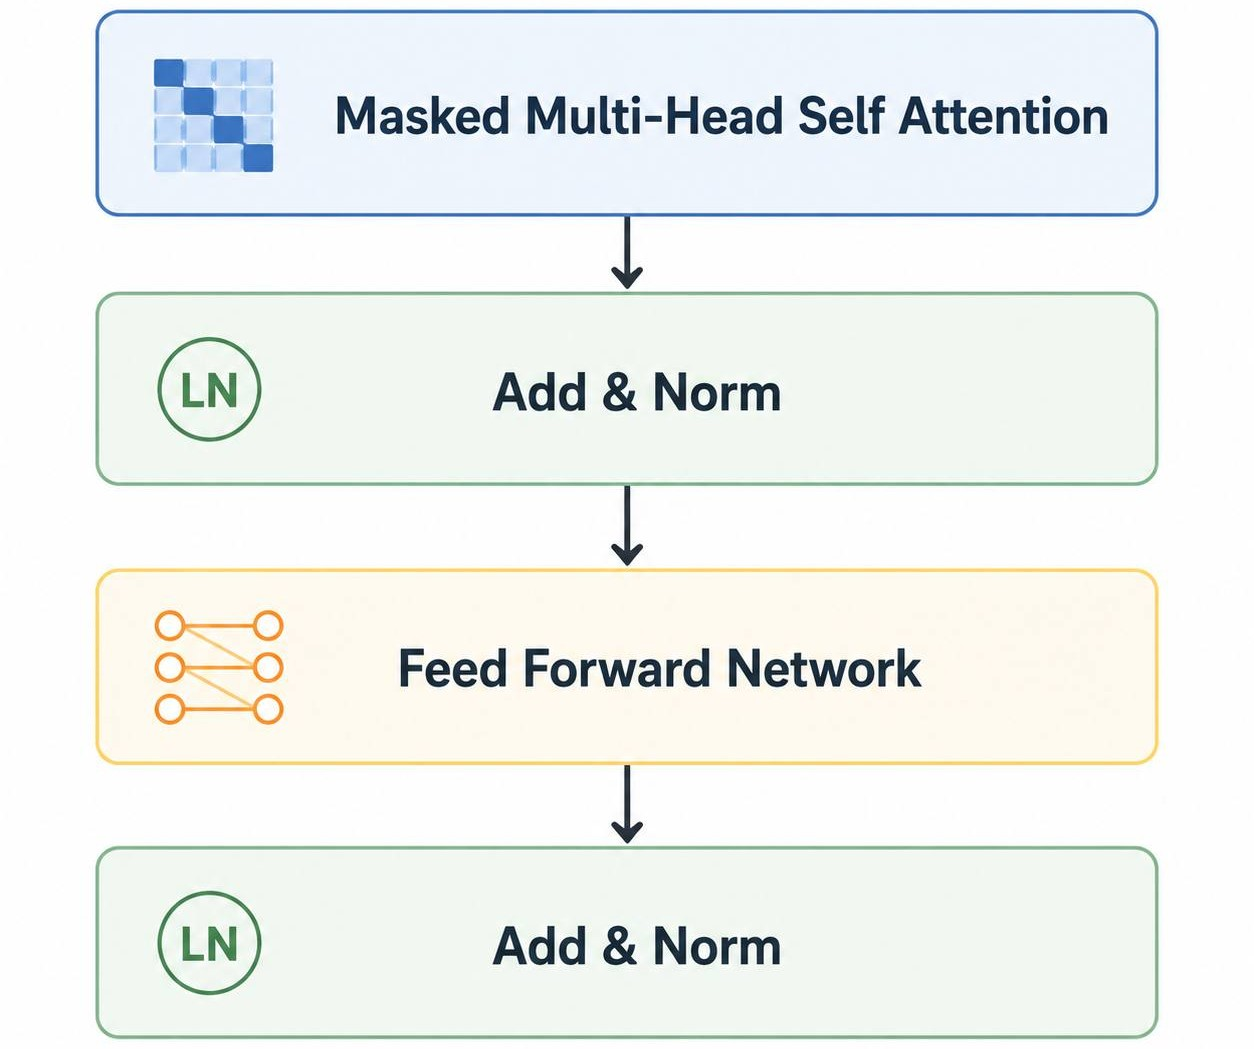
\includegraphics[width=0.95\textwidth]{figures/rnn3.jpg}
\end{figure}


This architecture is considerably simpler than The Original Transformer decoder while Preserving everything required for Autoregressive generation.

At first removing Cross-Attention might Seem like a loss of information. However, GPT does not require information from another Sequence. The Prompt itself becomes part of the decoder input, the Prompt itself provides the Context that would otherwise have been supplied by an encoder.

\subsection{GPT Input Architecture}

GPT converts raw text into numerical representations through tokenization, Vocabulary lookup, token embedding, and positional embedding:
\begin{equation}
E = E_{\text{pos}} + E_{\text{TokenEmb}}
\end{equation}
Unlike BERT, GPT uses only Token and Positional embedding because it Processes a single autoregressive sequence, while early GPT models relied on learnable absolute pos embedding, modern decoder-only models predominantly use Rotary Pos Embedding (RoPE) to Support long-context reasoning and improved positional Generalization.

\subsection{Training GPT}

Unlike traditional supervised learning, GPT does not Require labeled datasets. Instead, the model is trained On large text corpora Collected from sources such as: Books, wikipedia, Scientific Articles, News websites...

Through extensive Optimization over billions to trillions of Tokens, The Model learns General language representations, factual Knowledge, reasoning patterns, and Coding abilities. The resulting foundation model serves as The starting point for subsequent stages such as supervised fine-tuning\dots

\paragraph{Inference}
Autoregressive Generation is The inference Procedure used by GPT and other decoder-only language models. Starting from an input Prompt, The model predicts The one Token at a time, appends it to The Sequence, and repeats The Process until a stopping Condition is reached. Because each prediction depends on all previous tokens, inference is inherently Sequential. Efficient Generation relies on The KV cache.

\subsection{Decoding Algorithms}

After GPT computes The Probability distribution over the Vocabulary, it must choose which token to Generate next. This decision is performed by a decoding algorithm.

\paragraph{Greedy Search}
Always selects The Token with the highest probability. \\
\textit{Limitation:}
\begin{itemize}
    \item Often Produces repetitive Text
    \item Can miss better Overall Sequence
    \item Limited diversity
\end{itemize}

\paragraph{Beam Search}
Maintains the top-$k$ most probable partial Sequences. \\
\textit{Limitation:}
\begin{itemize}
    \item Computationally expensive
    \item Often Generates generic Response
    \item Rarely used in modern LLMs
\end{itemize}

\paragraph{Temperature Sampling}
Control the sharpness of The probability distribution before Softmax:
\begin{itemize}
    \item $0.2 - 0.5$: Factual tasks
    \item $0.7 - 1.0$: Balanced Generation
    \item $+1.2$: Highly Creative generation
\end{itemize}

\paragraph{Top-$K$ Sampling}
Instead of Considering the entire vocabulary, Top-$K$ sampling Keeps only the $K$ most probable tokens. The Remaining tokens receive probability 0, then performed only among these top-$K$ candidates.

\paragraph{Top-$P$ (Nucleus) Sampling}
Instead of Selecting a fixed number of Tokens, Top-$P$ Sampling selects The smallest set of tokens whose cumulative probability exceeds $p$. The candidate set changes dynamically depending On the probability distribution.

\paragraph{Typical Sampling}
Selects tokens whose information content is close to The expected entropy of the Probability distribution, it Prefers tokens that are statistically typical for The Current context.

\paragraph{Repetition Penalty}
During long generation, language models may Repeat words or phrases. A repetition penalty decrease the Probability of tokens that have already appeared in the Generated sequence. This encourages more varied and Coherent Outputs.

\subsection{Combined Decoding Strategies}

Most modern LLMs use a Combination of Decoding techniques rather than a Single algorithm. A Common Combination:
\begin{itemize}
    \item Temperature Sampling
    \item Top-$P$ Sampling
    \item Repetition Penalty
\end{itemize}

This combination provides a good balance between factual accuracy, fluency, and diversity.

\subsection{Best Decoder-Only Models}
\begin{itemize}
    \item ChatGPT
    \item DeepSeek
    \item Claude
    \item LLaMA
    \item Qwen
    \item Grok
\end{itemize}
